\documentclass[12pt, journal, onecolumn]{IEEEtran}
\usepackage[switch]{lineno}
\usepackage[utf8]{inputenc}
\usepackage{graphicx}
\usepackage{amsmath}
\usepackage{float}
\usepackage{caption}
\usepackage{url}
\usepackage{pdfpages}
\usepackage{setspace}
\usepackage{multicol}

\usepackage{tabularx}
\usepackage{booktabs}
\usepackage[colorlinks, citecolor=blue]{hyperref}
\usepackage[numbers, sort]{natbib}
\usepackage{others/aastex_hack}
\usepackage{subfloat}
\usepackage{siunitx}
\usepackage{aastex_hack}
\usepackage{xcolor}


\newcolumntype{C}{>{\centering\arraybackslash}X} % centered version of "X" type
\setlength{\extrarowheight}{1pt}
\DeclareSIUnit{\parsec}{pc}
\DeclareSIUnit{\yr}{yr}

\newcommand{\kpc}{\kilo\parsec}
\newcommand{\lowalpha}{low-$[\alpha/\text{Fe}]$}
\newcommand{\highalpha}{high-$[\alpha/\text{Fe}]$}
\newcommand{\feh}{[\text{Fe}/\text{H}]}
\newcommand{\mone}[1]{m_{1_{\text{#1}}}}
\newcommand{\mtwo}[1]{m_{2_{\text{#1}}}}
\newcommand{\semaxis}[1]{a_{\text{#1}}}
\newcommand{\ecc}[1]{e_\text{#1}}
\newcommand{\interval}[1]{t_\text{#1}}

\if
CLASSINFOpdf
\else
\fi

\title{Detecting gravitational waves sources $-$ BHBH, NSNS, BHNS $-$ with LISA}
\author{
    \IEEEauthorblockN{Nazeela Aimen},
    \IEEEauthorblockN{Syed Ali Mohsin Bukhari},
    \IEEEauthorblockN{Asad Ali}
    \and\\
    \IEEEauthorblockA{
        \textit{
            Department of Applied Mathematics and Statistics, Institute of Space Technology, Islamabad 44000, Pakistan.
        }\\
    }
    \IEEEauthorblockA{
        \textit{
            Space and Astrophysics Research Lab (SARL), Institute of Space Technology, Islamabad 44000, Pakistan.
        }
    }
}

\markboth{Journal of- \LaTeX\ Class Files,~Vol.~14, No.~8, August~2015}%
{Shell \MakeLowercase{\textit{et al.}}: Bare Demo of IEEEtran.cls for IEEE Journals}

\begin{document}
    \bstctlcite{IEEEexample:BSTcontrol}
    \maketitle
    \IEEEpeerreviewmaketitle
    \begin{abstract}
        \, \color{red}{Abstract is still missing!!}
    \end{abstract}
    \begin{IEEEkeywords}
        Cobb-Douglas Habitability Score, Exoplanets, Habitability, Habitable zone, Convex Optimization, Duality.
    \end{IEEEkeywords}

    \linenumbers


    \section{Introduction}
    \label{sec:intro}
    The gravitational waves (GW) were predicted a year after the final formulation of the general theory of relativity (GR) by Albert Einstein~\cite{Einstein1916}.
    Similar to electromagnetic waves, the GWs travel at the speed of light~\citep{Eddington1922, Abott2017}.
    However, unlike electromagnetic waves, the GW stretches and squeezes the space itself thus causing spatial disturbances.
    The detection of Hulse-Taylor binary~\citep{Hulse1975}, and the subsequent observation of a seven years time
    span~\citep{Taylor1982} stirred a great interest in the GW observations.
    It wasn't until 2015 that the first direct observation of GW was made by LIGO and VIRGO collaborations~\citep{Abott2017}.
    The lower frequency bound for both the aLIGO and VIRGO detectors is around \SI{10}{\hertz}~\cite{aLIGO2015, aVIRGO2014}

    The Laser Interferometer Space Antenna (LISA) has three spacecrafts that form a triangle, each side 2.5 million
    km long~\cite{Prince2002, Robson2019}.
    Operating in the frequency range of \SI{1e-5}{\hertz}$\,\leq  f \leq\,$\SI{1e-1}{\hertz} LISA will be able to observe the sources millions of years before they merge.
    The early detection capability will help better constrain and determine the orbital parameters of the observed binaries.
    Some sources detectable by LISA are the extreme mass ratio inspirals (EMRIs)~\cite{Gair2017, Klein2016, Chapman2022} and galactic binaries~\cite{wagg2021gravitational, Abott2017, Digman2022}.
    This makes LISA also capable of mapping Milky Way galaxy's structure.
    Another interesting class detectable by LISA is the double white dwarf stars (DWDs) which are reported to be abundant in our MW galaxy and have a substantial detection in LISA as well~\cite{Korol2017, Nelemans2001, Willems2007, Ruiter2010}.


%    The system  of the problem in which HZ and CDH are explained in Section~\ref{sec:sm}, while sections~\ref{sec:r} and~\ref{sec:df} describe results, and discussion and future work respectively.

    A lot of effort has been put into the detection of potential GW sources for LISA, the resolution of issues that might be associated with the background data, and proposals of new candidates as GW sources for LISA~\cite[see, for example,][]{Lau2020, Sesana2009, Khakhaleva2020, Renzo2021, Fumagalli2022, wagg2021gravitational, Broekgaarden2021, Shao2021, Andrews2020, Belczynski2010, Guo2017, Babak2010, Blaut2010, Babak2008, Ruiter2010, Nelemans2001, Yu2010}.
    The detections of these sources will provide us with a better understanding of not only the evolution phases but also the endpoints of stellar evolution.

    The goals of this research are,
    \begin{itemize}%
        \item to predict the number of DCO binaries that can be detected via LISA in our Milky Way galaxy,
        \item to determine whether extra galactic sources are LISA detectable,
        \item to make a general detection comparison between DCO binaries with and without an initial eccentricity.
    \end{itemize}%

    For this purpose, we generate the binaries using COMPAS, section~\ref{sec:population_synthesis}.
    One hundred random Milky Way (MW) instances were generated in which the binaries were placed for detection, section~\ref{sec:milky_way}.
    The detection of the binaries was done using LEGWORK v0.3.0~\cite{wagg2021legwork}.\footnote{\url{https://github.com/TeamLEGWORK/LEGWORK/tree/v0.3.0}}


    \section{Population synthesis}
    \label{sec:population_synthesis}
    The population synthesis for the detections of the double compact objects (DCOs) was performed using the Compact Object Mergers: Population Astrophysics and Statistics (COMPAS; ~\cite{stevenson2017formation, Riley2022, Vigna2018}) suite.
    COMPAS is a rapid stellar evolution suite and can evolve both single and binary stars following the details outlined by~\cite{Hurley2000, Hurley2002}.
    A list of selected papers that make use of the COMPAS suite is also available on the COMPAS website.\footnote{\url{https://compas.science/science.html}}

    This study makes use exclusively of the binary star evolution (BSE) synthesis method.
    The default parameters used by the COMPAS software are listed in table 1 in the COMPAS paper~\cite{Riley2022}.

    Except for supernova mass remnant prescription, initial eccentricity ($e_i$), metallicity ($z$), and pulsar evolution, all other parameters were taken at the default value.
    For a one-to-one correspondence between the two generated data sets, the seed numbers were kept constant.

    For the mass of primary star, we draw the values from Kroupa initial mass function (IMF) with $m_1 \in [5, 150]\,\text{M}_\sun$~\cite{kroupa2001variation}.
    For the secondary star, we randomly draw from uniform distribution to satisfy $q\equiv m_2/m_1$, where $q\,\in\,[0, 1]$~\cite{sana2012binary}.
    An additional constraint of $m_2 \geq 0.1\,m_1$ was placed on $m_2$ as this is the minimum mass necessary for a star to be considered as a main sequence star.

    For the semi-major axis of the binary, we drew the parameter values from a flat-in-the-log distribution with $a_i \in [0.1, 1000]\,$AU, such that $p(a_i) \propto 1/a_i$~\cite{opik1924photographic}.

    For the remnant mass prescription, we first considered the Fryer delayed model~\cite{Fryer2012}.
    However, this resulted in a concentration of NS mass around $\sim1.28\,\text{M}_\sun$.
    To avoid this concentration of NS final mass, we used Müller \& Mandel prescription (M\&M)~\cite{Mandel2020}.
    M\&M is a stochastic remnant mass model that offers a smoother mass distribution for NS\@.
    We also switched the \textbf{evolve\_pulsar} flag to \textbf{True} during population synthesis.

    For metallicity, we drew the values from a $\text{Beta}(5, 80)$ distribution.
    The main motivation behind the selection of such biased distribution is the higher metallic content of present-day stars.
    The population III stars were primarily composed of pure hydrogen and their deaths produced heavier metals in the Universe.
    By this extension, the stars that are present now or those that will merge now must have higher metallic content.
    As such, we also note that having stars with higher metallic content might produce more NSNS or NS-BH pairs for detection.

    For eccentricity, we make use of two cases,
    \begin{itemize}
        \item Case I: All the binary systems are generated using a flat distribution, $e \in [0, 1]$.
        \item Case II: All the binary systems are generated with circular orbits, i.e., $e = 0$.
    \end{itemize}

    Details about the selection of metallicity and eccentricity values in COMPAS are provided in appendix~\ref{sec:appA}.


    \section{Milky way Model}
    \label{sec:milky_way}
    In this section, we will briefly outline the milky way galaxy model used in this study.
    The model is developed by~\cite{wagg2021gravitational} and makes use of the galaxy's enrichment history by taking
    into account the metallicity-radius-time relationship~\cite{Frankel2018}.
    It uses a separate star formation history and spatial distribution for the \lowalpha, \highalpha\ discs, and bulge in the galaxy.

    \subsection{Star formation rate}
    \label{subsec:star_formation_rate}
    The star formation rate for both the \lowalpha\ and \highalpha\ disks is expressed as,
    \begin{equation}
        p(\tau) \propto \exp\left(-\frac{\tau_m - \tau}{\tau_\text{SFR}}\right),
        \label{eq:star_formation_rate_equation}
    \end{equation}
    where $\tau$ is the time difference between the star's ZAMS stage and today.
    The age of milky way galaxy, $\tau_m$, is taken as \SI{12}{\giga\yr}, and the star formation rate as, $\tau_\text{
        SFR}\ $= \SI{6.8}{\giga\yr}.
    The star-forming period of \lowalpha\ and \highalpha\ discs were taken as \SIrange{0}{8}{\giga\yr} and \SIrange{8}{12}{\giga\yr} respectively.
    The model adopts \SIrange{6}{12}{\giga\yr} as the star-forming period of the bulge~\cite{Bovy2019}.

    \subsection{Radial distribution}
    \label{subsec:radial_distribution}
    The radial distribution of stars within the milky way galaxy was performed using the following expression,
    \begin{equation}%
        p(R) = \exp\left(-\frac{R}{R_d}\right)\frac{R}{R_d^2}
        \label{eq:radial_distribution_of_stars}
    \end{equation}%

    However, a different scale length, $R_d$, was chosen for each component of the galaxy.
    For \lowalpha, the model uses $R_\text{exp}(\tau)$ as the scale length~\cite[Eq 6]{Frankel2018}, where

    \begin{equation}%
        R_\text{exp}(\tau) = 4\,\text{kpc}\left[1 - \alpha_{R_\text{exp}}\left(\frac{\tau}{8\,\text{Gyr}}\right)\right],
        \label{eq:exponential_radius_equation}
    \end{equation}%
    with the value of inside-out growth parameter, $\alpha_{R_\text{exp}}$, as 0.3. For \highalpha\ disc and bulge, the value of scale length was chosen as $(1/0.43)\,$\si{\kpc} and \SI{1.5}{\kpc} respectively.

    \subsection{Vertical distribution}
    \label{subsec:vertical_distribution}
    The model employs a similar method of single exponent expression with varying scale height parameters for the vertical distribution as well.
    The exponential expression used is,
    \begin{equation}
        p(|z|) = \frac{1}{z_d}\exp\left(-\frac{z}{z_d}\right),
        \label{eq:vertical_distribution_of_stars}
    \end{equation}
    where $z$ here is the vertical displacement from the galactic plane.
    The scale height parameter, $z_d$, for \lowalpha, \highalpha\ and bulge was taken as \SI{0.3}{\kpc}~\cite{McMillan2011}, \SI{0.95}{\kpc}~\cite{Bovy2016}, and \SI{0.2}{\kpc}~\cite{Wegg2015} respectively.

    \subsection{Metallicity-radius-time relationship}
    \label{subsec:metallicity_radius_relationship}
    The MRT relationship plays an important part, both in the galaxy model and later on in the placement of DCOs within the galaxy as well.
    The model makes use of~\cite[Eq. 7]{Frankel2018},
    \begin{equation}
        \begin{aligned}
            \feh(R,\tau) = {} & F_m + \nabla\feh R - \left(F_m + \nabla\feh R_{\feh=0}^{\text{now}}\right) f(\tau)
        \end{aligned}
    \end{equation}

    \subsection{Galaxy synthesis}
    \label{subsec:galaxy_synthesis}
    For the synthesis of an instance of the Milky Way galaxy, the model described previously samples the following parameters,
    \begin{equation*}
        \theta_i = \{\tau, D, z, \text{component}\},
    \end{equation*}
    where $\tau$ is the look-back time for the binary, $D$ is the distance from Earth, $z$ is the metallicity, and `component' is the component of the galaxy in which the binary resides.\footnote{One of the three, \lowalpha\ disc, \highalpha\ disc, or bulge.}
    The parameters are generated for $i = 1, 2, 3, \ldots$, $N_\text{GAL}$, where $N_\text{GAL} = 100$.
    For each galaxy generated, all the COMPAS generated DCOs were tested for their detection.
%    The method for detection is described in section~\ref{subsec:detection}.


    \section{Parameters of interest}
    \label{sec:parameters-of-interest}
    We first generated \num{1e7} values for metallicity using the beta distribution within the COMPAS limits (see, appendix~\ref{sec:appA} for details).
%    The values were stored in ten separate grid files and used with COMPAS to simulate the binaries.
    We denote the zero-age main sequence (ZAMS) parameters of the binaries as,
    \begin{equation}%
        \mone{ZAMS}, \mtwo{ZAMS}, \semaxis{ZAMS}, \ecc{ZAMS}, Z, \o
        \label{eq:zams_parameter_names}
    \end{equation}%
    COMPAS evolves the binaries up to \SI{13.7}{\giga\yr}.
    We represent the resulting double compact object (DCO) parameters as,
    \begin{equation}%
        \mone{DCO}, \mtwo{DCO}, \semaxis{DCO}, \ecc{DCO}, \interval{evolve}, \interval{inspiral}, Z, \o,
        \label{eq:dco_parameter_names}
    \end{equation}%
    where $Z$ is the metallicity of the binary system, $\o$ is the seed number, $\interval{evolve}$ is the time required to form DCO from ZAMS, and $\interval{inspiral}$ is the DCO in-spiral time. $\semaxis{ZAMS}$, $\semaxis{DCO}$, $\ecc{ZAMS}$, and $\ecc{DCO}$ are the semi-major axis and eccentricity of the binary orbit at ZAMS and DCO formation respectively.
    \begin{figure}[!ht]%
        \centering
        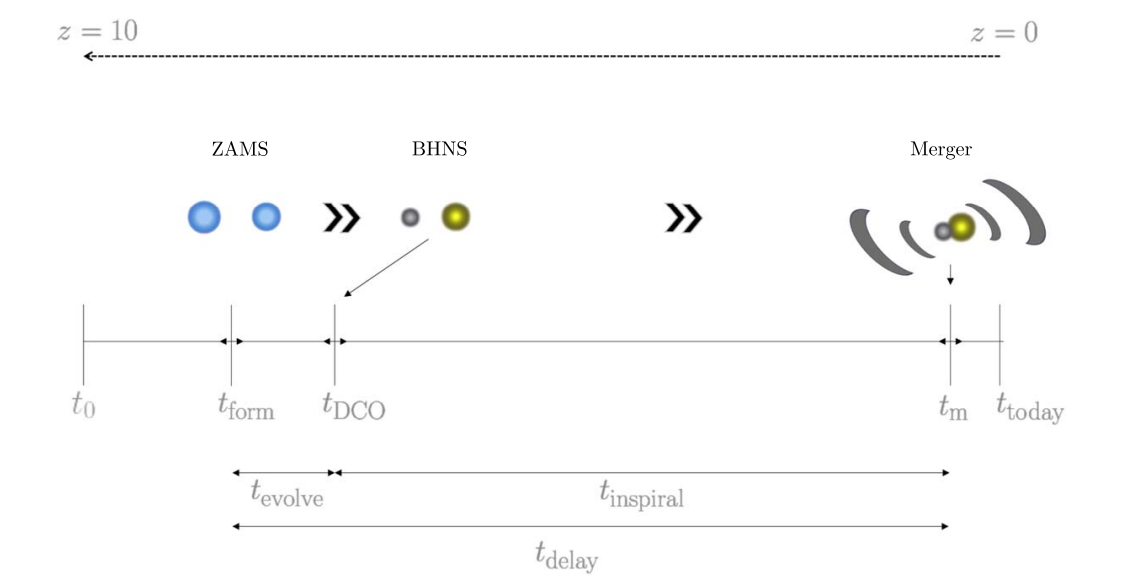
\includegraphics[width=\linewidth]{images/binary_evolution}
        \caption{Schematic diagram showing various time intervals for a binary system from ZAMS formation, to DCO, and merger. The figure is taken from~\cite{Riley2022}.}
        \label{fig:binaryevolution}
    \end{figure}%
    These parameters were then provided to the python framework LEGWORK~\cite{wagg2021legwork} that evolved these binaries from the DCO stage to the merger state.
    It evolves the binaries using equations from~\cite{Peters1963, Peters1964}.
    The detection is made based on the signal-to-noise ratio (SNR) of the binary averaged over sky position, polarization, and orientation using the following expression from~\cite{Finn2000},
    \begin{equation}
        \rho^2 = \sum_{n=1}^{\infty}\int_{f_{n, i}}^{f_{n, f}}\frac{h_{c, n}^2}{f_n^2 S_n(f_n)}\,\text{d}f_n,
        \label{eq:snr_equation}
    \end{equation}
    where $n$ is the GW harmonic, $f_n$ represents the orbital frequency of $n^\text{th}$ harmonic.
    The parameter $S_n(f_n)$ is the LISA sensitivity curve function~\cite{Robson2019}, and $h_{c, n}$ is the characteristic strain of the $n^\text{th}$ GW harmonic~\cite{Barack2004}.
    \begin{equation}
        h_{c,n}^2 = \frac{2^{5/3}}{3\pi^{4/3}}\frac{(G\mathcal{M}_c)^{5/3}}{c^3 D_L^2}\frac{1}{f_\text{orb}^{1/3}}\frac{g(n, e)}{nF(e)}
        \label{eq:characteristic_strain}
    \end{equation}


    %\subsection{Binary Evolution}\label{subsec:be}
    %One of the most important factors in the observation of any source is their distance from the observational instrument.
    %As it is a known fact that for all the sources, we can observe their past depending upon how far are we from it.
    %This surely complicates the evolution of our DCO as at the time of observation, LISA will also be observing the past of the sources.
    %To handle such a situation, we first calculate the time the GW will take from the source to LISA using the given distances within the milky way.
    %This logic is implemented within Legwork~\cite{wagg2021legwork} which gives strong tools for evolving the sources to the desired point.

    \section{Reults 1: COMPAS sources}
    In this section we discuss the DCO pairs obtained via simulation in the COMPAS suite.


    \section{Results 1: LISA Sources}
    \label{sec:r}
    \begin{subfigures}
        \begin{figure*}[!t]
            \centering
            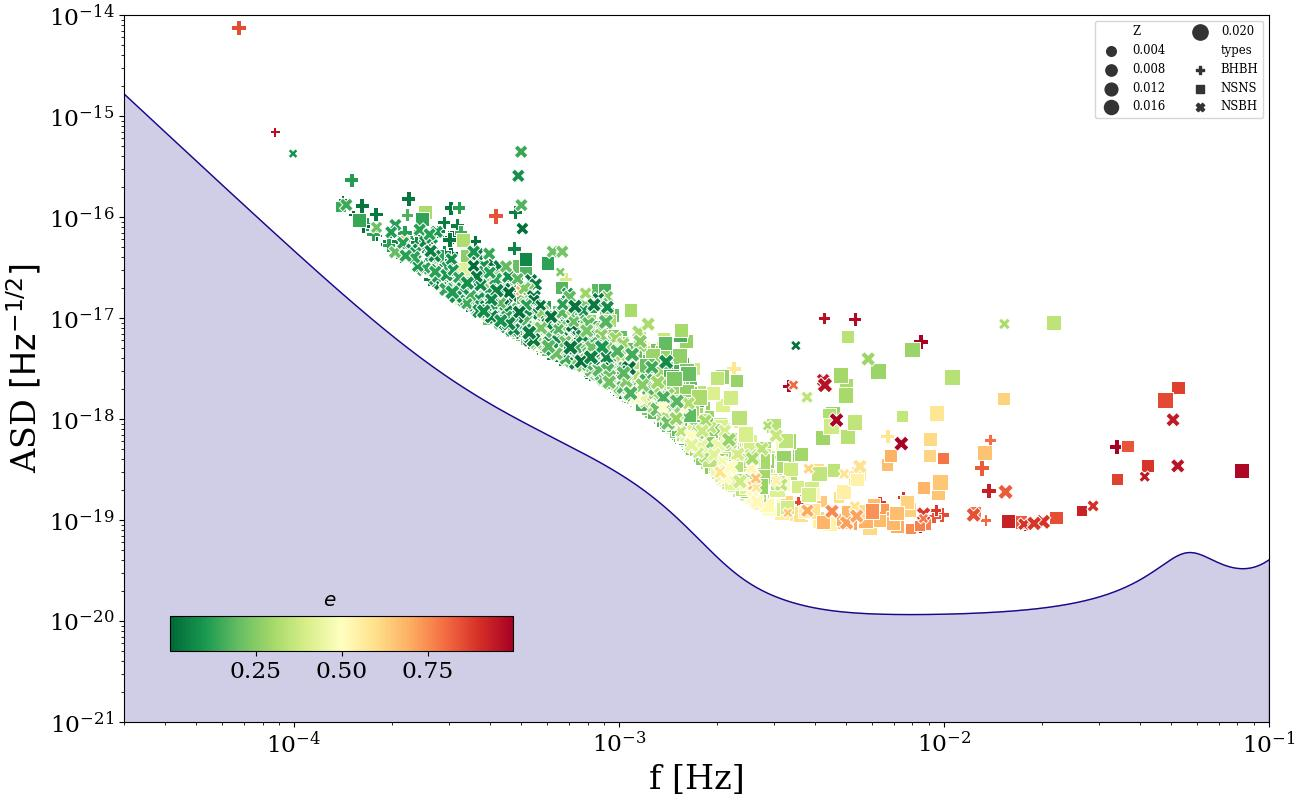
\includegraphics[width=0.82\linewidth]{images/first}
            \caption{\label{first}Detectable sources' characteristic strain along with dominant frequency in our simulations (Top) is shown on the LISA sensitivity curve as well as their separate types (bottom). The sources are placed based on their eccentricities i.e. Highly eccentric sources are towards the red side while low eccentric sources are on the green side of the spectrum. The reference lines are based on the average eccentricity of our simulations i.e. where in the galaxy an eccentric binary would be assuming an average chirp mass, orientation, and sky location for a remaining inspiral time (vertical lines) and a given distance (diagonal lines). See also figure bla bla for detail understanding.}\label{detect} %--> Fig.1a
        \end{figure*}
        \begin{figure}
            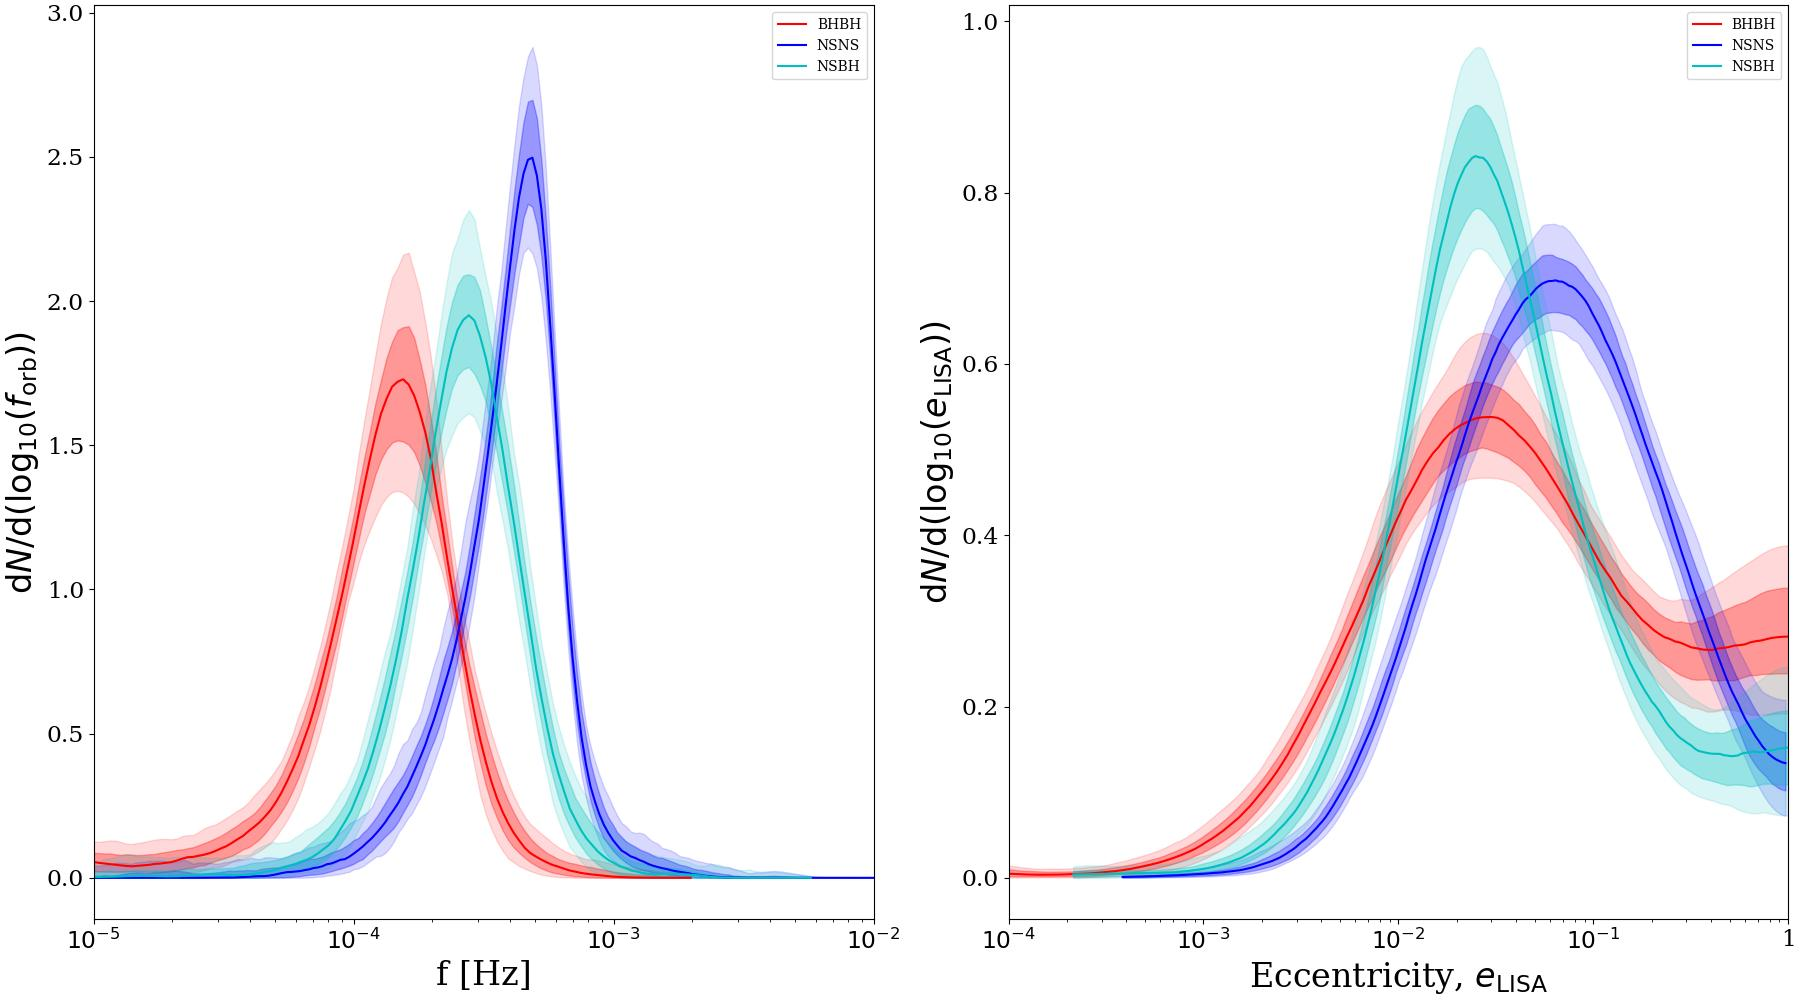
\includegraphics[width=\linewidth]{images/second}
            \caption{Caption text.}\label{fig:freq} %--> Fig.1b
        \end{figure}
    \end{subfigures}

    This section contains our findings and results, comprising the predictions of the given types of DCOs for LISA in the Milky Way and a detailed analysis of their properties.
    Based on our fiducial model, we expect in total $4.7\times 10^{-3}\%\,(186.41)$ detections on average in a $4\,(10)$ years LISA mission in which $1.39\times 10^{-3}\%\,(108.35)$, $1.4\times 10^{-3}\%\,(6.68)$, $1.91\times 10^{-3}\%\,(34.94)$ are BHBH, NSBH, and NSNS respectively.
    Moreover, we also plot our detectable sources concerning the LISA sensitivity curve (figure~\ref{detect}) in section~\ref{subsec:r11}. \textbf{Tell the summary of the rest of the results here.}

    While this section comprises detailed analysis of our fiducial model, section~\ref{sec:ecc} describes the comparison of
    eccentricity-based simulations.

    \subsection{Population of Detectable sources} \label{subsec:r11}
    The predicted distribution of the LISA detectable sources is plotted over its expected sensitivity curve, containing the galactic double white dwarf population noise~\cite{Robson2019}, in figure~\ref{detect}.
    The x-axis of the graph is the GW frequency.
    For the circular binaries in our data, the GW frequency is $2f_\text{orb}$ is the correspondence for the x-axis.
    We take the dominant frequency, the frequency accumulating the largest SNR, for the eccentric binaries.
    Furthermore, the y-axis stipulates the amplitude spectral density (ASD), including the contribution from all harmonics.

    The gap between the detected binaries and the LISA curve in the graph is the SNR criteria, ($\text{SNR}\,>\,7$). Furthermore, the binaries are shaped based on their type; plus, square, and cross show BHBH, NSBH, and NSNS, respectively.
    The size of the points varies with metallicity; high metallic sources have larger shapes than low metallic ones.
    The color scheme for the binaries is based on the eccentricity strength of the detected binaries, shown through a color bar at the bottom left in the plot.
    For example, the red ones are the most eccentric sources, the yellow ones are mid-eccentric, and the green ones are the sources with low eccentricities.

    Around $3\,\text{mHz}$, some binaries mostly have large eccentricities.
    These are on the right side of the graph and extend downwards to $10^{-19}$ ASDs. However, there are also some BHBH that are almost circular and emit at high frequency.
    These sources are in their last stages of merger hence they are spinning fast enough to emit large frequency GW\@.

    The major binary population is concentrated on the left side of the LISA sensitivity curve.
    The peak of concentration around the GW frequency of \textbf{0.12 mHz}.
    The main reason for such a trend can be explained through the eccentricities of the binaries.
    As seen from the figure~\ref{detect}, a large population of our binaries are low eccentric or mid-eccentric.
    There are also binaries having high eccentricities which as mentioned above lie on the right side of the graph.
    The orbit of low eccentric or circular binaries evolves differently than high eccentric binaries.
    After the formation of DCO, most of the low eccentric binaries emit GW in low-frequency bands of LISA as the orbit progresses.
    While DCOs with high eccentricities behave in a completely different way, i.e.\ their orbit decay faster, and they tend to emit GW in the high-frequency LISA detection band.
    Although these are of prime importance in the LISA mission, unfortunately, these are rare.
    Thus, most of the DCOs are at lower frequency regions.

    Fig.~\ref{fig:freq} shows the distribution of the orbital frequency; $f$, and eccentricity at the time of LISA mission; $e$.
    The regions surrounding the individual graphs are the $1\,\sigma$, and $2\,\sigma$ uncertainties which are the variations of the results over 100 random instances of our galaxy.
    We plot this figure using the bootstrapping function~\cite{wagg2021gravitational}.
    The left side of the graph is the orbital frequency distribution.
    It shows peaks of different types of sources i.e. \textbf{0.3mHz, 0.7mHz, 0.99} for BHBH, NSNS, and NSBH\@.
    The reason for such a trend is because of the mass difference as higher mass DCO The distribution is a little negatively skewed.
    As mentioned above, a higher mass DCO at the same distance and eccentricity requires a lower frequency to produce the same signal-to-noise ratio and thus be detected.
    The orbital frequency distributions for BHBHs, BHNSs, and NSNSs (figure, 3a) peak at progressively increasing
    frequencies as mentioned in section 3.1.
    The distributions appear nearly symmetric, but closer inspections show that the left-hand side is more populated, which can be seen most clearly in the curve for the BHBHs.
    This is due to the contribution of highly eccentric binaries, which are most abundant in the BHBH population.
    These systems are still detectable by LISA, despite their low orbital frequency, as the high eccentricity means that the majority of the GW signal is emitted at higher harmonics, where LISA is more sensitive.

    We can also observe the peaks for high chirp mass systems have peaks in the low-frequency detection region, as they emit the waves in lower frequency.
    Hence, this is another way to differentiate sources.
    Hence, the BHBH pairs have the most eccentric pairs having the highest average eccentricity and $\langle M_c\rangle$.

    \subsection{Detections in Components}\label{subsec:detectionetections-in-components}
    Our simulated galaxy comprises three components; Low $\alpha$ disc, High $\alpha$ disc, and Bulge.
    Figure~\ref{fig:pie1} describes the average distribution of detectable sources in these components.
    The average total number of detections are in shown in the middle.
    BHBH, having a significant number of detections, is equally distributed in the low$-\alpha$ disc and high$-\alpha$ disc, while the rest have slightly more detections in the latter than prior.
    Bulge has the least number of detected DCOs.
    Thus, there is a high probability for LISA to detect GW sources in the two components.

    \begin{figure}
        \centering
        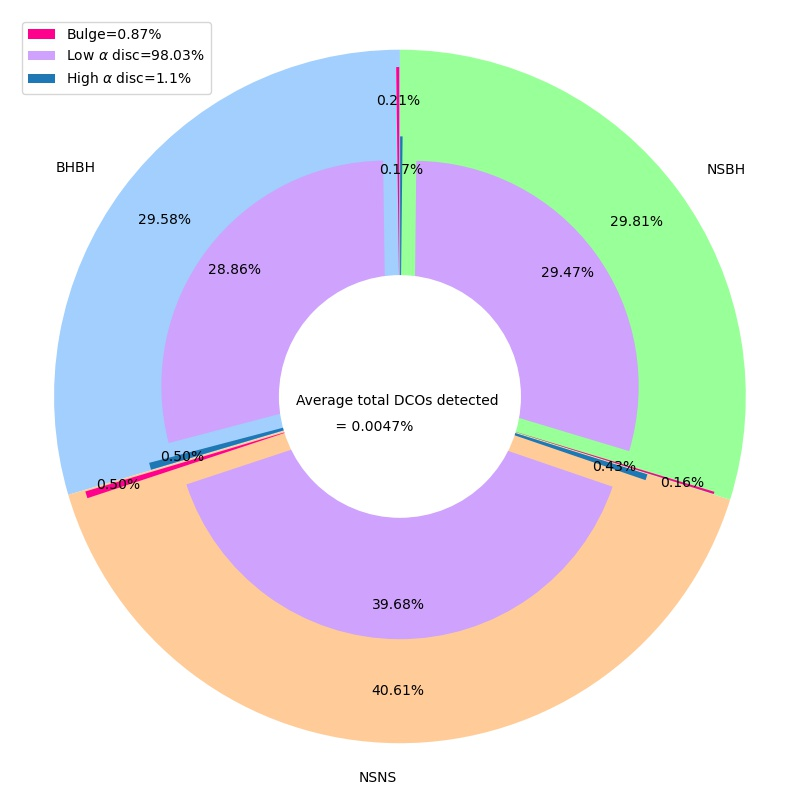
\includegraphics[width=\linewidth]{images/pie_chart}
        \caption{Average detectable sources distribution in three components of simulated milky way}
        \label{fig:pie1}
    \end{figure}

    \subsection{Maximum distance}\label{subsec:maximum-distance}
    For each DCO, there is a horizon distance i.e., the maximum distance up to which the DCO may be detectable in
    LISA. This is calculated using the inverse relationship between SNR ($\rho$) and distance~\cite{Lau2020},
    \begin{equation}
        \label{eq:eq1}
        d_\text{max}=\frac{\rho(d\,=\,1\,\text{kpc})}{\rho_\text{min}}
    \end{equation}

    Where $\rho_{\min}$ is the minimum value of SNR below which the source is not detectable.
    We keep the detection threshold at $\rho_{\min}\,=\,7$, and $\rho(d\,=\,1\,\text{kpc})$ is SNR of the source if it was at $1\,\text{kpc}$ distance from the detector.
    We calculated the SNR of all the detected sources at \SI{1}{\kpc} distance using the python package LEGWORK~\cite{wagg2021legwork}.
    Afterward, their maximum distances $(d_{\max})$ were calculated.

    Figure~\ref{fig:dmax} shows the maximum distances for all the detected sources.
    The top shows $d_{\max}$ for BHBH, and NSNS while the bottom has NSBH and BHNS\@.
    These are calculated for all the LISA band frequencies.
    The black line shows the average maximum distance for all the types.
    The LISA sensitivity curve is also overlaid on the graph as a blue line.

    BHBH, being the dominant source can be observed to an average distance of more than \SI{1e5}{\kpc}.
    NSBH and BHNS have almost the same average $d_{\max}$ i.e between \SI{1e3}{\kpc} and \SI{1e4}{\kpc} while NSNS has peak at $\sim\,$\SI{1e3}{\kpc}.
    The red dotted lines illustrate some known galaxies to have a better understanding of distances.
    Hence, BHBH can be discovered as far as Hoag's Object, NSNS in M31, and both BHNS and NSBH are far from M31 but much below Hoag's Object.


    Almost all the highest values of average $d_{\max}$ of four types are around a \textbf{certain frequency} i.e., if a source has \textbf{certain orbital frequency} then it can be detected to its maximum detection distance.
    It can be observed through the LISA overlay that this frequency lies in the area where the detector is most sensitive.
    Hence, if a source emits in the frequency region of the highest sensitivity of LISA, then it will be detected at a maximum distance.

    \begin{figure}
        \centering
        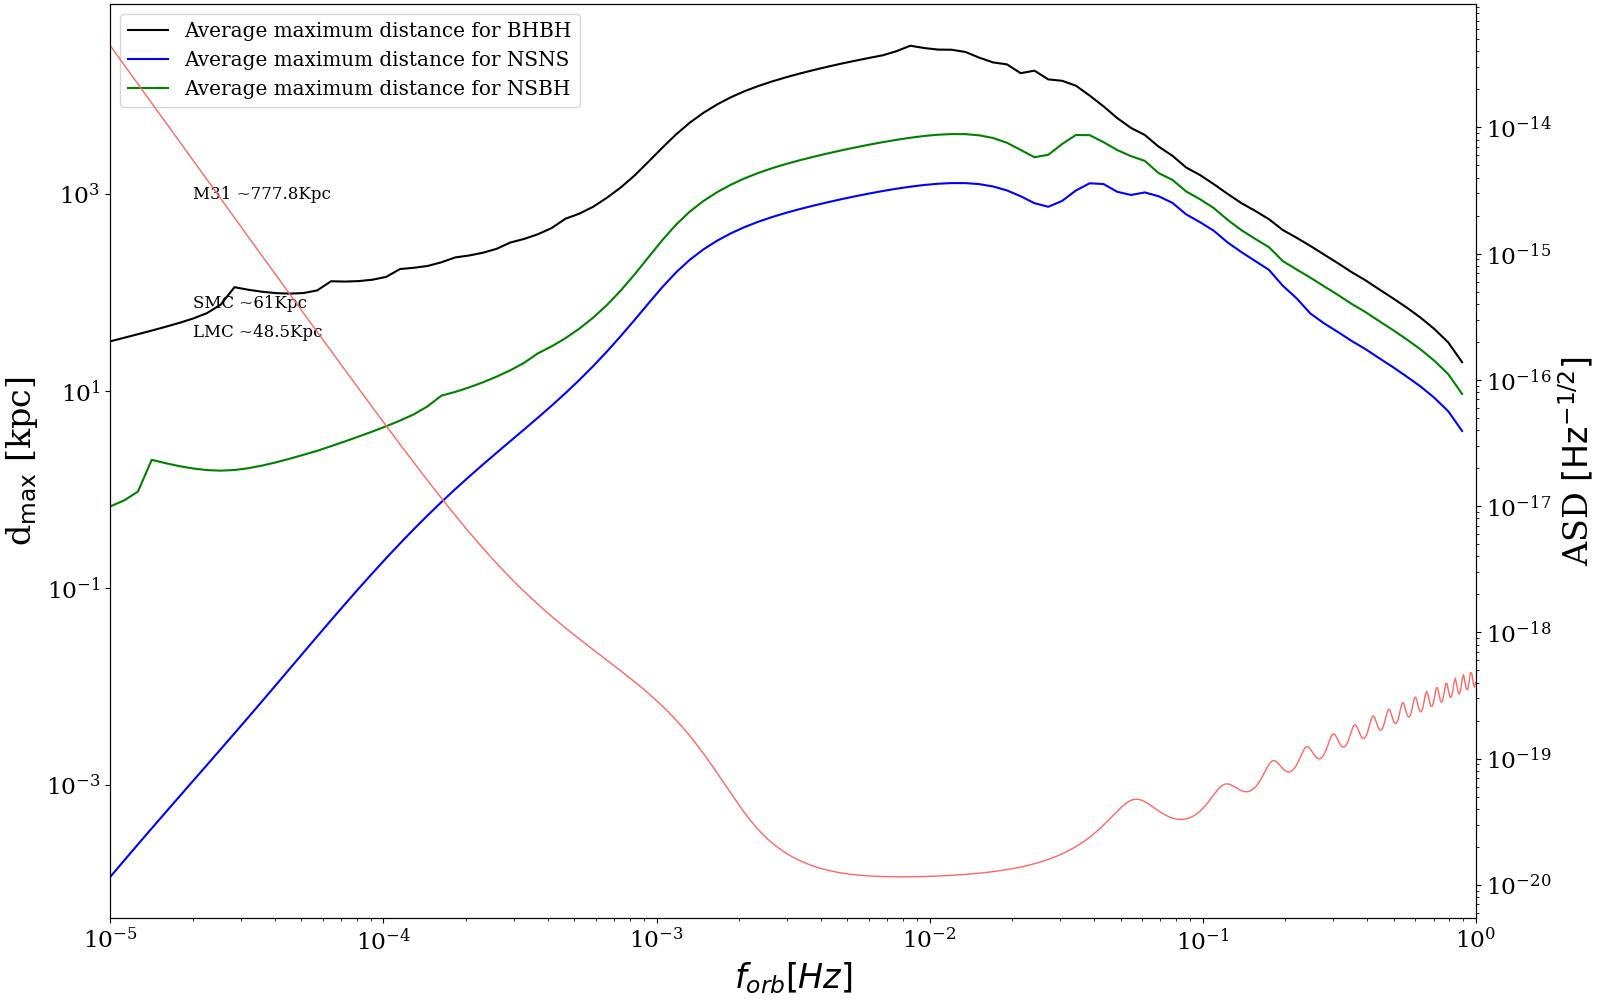
\includegraphics[width=\linewidth]{images/DMAX}
        \caption{Maximum distances for all of the different types of DCO. The average maximum distance is
        shown through a black line while the blue line shows the overlaid LISA sensitivity curve}
        \label{fig:dmax}
    \end{figure}


    \section{Results 2: Influence of Eccentricity}\label{sec:ecc}
    In this section, the outcomes of varying eccentricity at ZAMS are discussed.
    For this we use the same grid of parameters used in the fiducial model, however, the eccentricity is taken 0 at ZAMS (E0) instead of variable (VE).

    Firstly, the detection rates and predictions for different sources are discussed.
    Afterward, changes in observable properties are discussed.

    \subsection{Detection rates}\label{subsec:detectionetection-rates}
    The prediction for VE is a total of 136 detections in a 4 years LISA mission.
    A decrease in the detection rate is observed for E0 which is detected in a 4 years LISA mission.
    As there is no difference in any parameter other than eccentricity, then it is surely the root cause of the decline in detections.

    The difference in different types of sources is shown in the pie chart in which there is a clear reduction in the detected sources. \textbf{Explain the pie chart more}

    %\begin{figure}
    %    \centering
    %    \includegraphics[width=\linewidth]{pie_e0_evar.jpg}
    %    \caption{Comparison of detection rate in VE and E0.}
    %    \label{pie}
    %\end{figure}

    \subsection{Model variation: To be added somewhere else,}
    \label{subsec:model_variation}
    In a number of previous works, $e_\text{ZAMS}$ was taken as zero~\cite{Vigna2018, Barrett2018, Lau2020,
        Broekgaarden2021, wagg2021gravitational}.
    The main reason for this assumption is that they argue that eccentricity at ZAMS is not likely critical for predicting detection rates as they deal with post-interaction binaries and their orbital eccentricities become zero after mass transfer~\cite{Hurley2002}. %, de2015merger}).
    To test the accuracy of this assumption, we simulate another population with the same parameters.
    The only change is that $e_\text{ZAMS}$ of the binaries is left to be varied by the COMPAS suite.
    We compare the difference in detection rates and properties of the two models and give our conclusion.




    \section{Discussion and Future work}\label{sec:df}
    \ifCLASSOPTIONcaptionsoff
    \newpage
    \fi

%    \begin{IEEEbiographynophoto}{Nazeela Aimen}
%        Currently enrolled as an MS Mathematics student at the Institute of Space Technology (IST), Islamabad, Nazeela is a Gravitational wave research enthusiast.
%        She did her B.S in Space Science from the Institute of Space Technology (IST).
%        She is currently doing research on Particle Swarm Optimization in coherent all-sky search for gravitational wave detectors.
%    \end{IEEEbiographynophoto}

    \cleardoublepage
    \bibliographystyle{IEEEtran}
    \bibliography{reference}

    \cleardoublepage
    %	\onecolumn
    \appendices
    \section{Settings for using COMPAS}
\label{sec:appA}
To generate a binary system in COMPAS, we require the following parameters as discussed earlier,
\begin{itemize}
    \item mass of primary star $(\mone{ZAMS})$,
    \item mass of secondary star $(\mtwo{ZAMS})$,
    \item semi-major axis of the orbit $(\semaxis{ZAMS})$,
    \item random seed $(\o)$
    \item remnant mass prescription,
    \item eccentricity of the orbit $(\ecc{ZAMS})$, and
    \item metallicity of the stars $\left(Z\right)$.
\end{itemize}

We've discussed the first four parameters in the main text, here we will discuss the selection of eccentricity and metallicity values.

\subsection{\textbf{Eccentricity}}
\label{subsec:eccentricity}
In order to evaluate whether the initial eccentricity affects GW emission at the end stages of the DCO, we generate two identical data sets.
For the primary data set, we chose the eccentricity value to be varied between 0 and 1.

For the secondary data set, we assumed all the binaries to have circular orbits.
For cross-checking purposes we made sure to use the same seed numbers when generating the second data set that were used with the primary data set.
This enabled us to check the effects of initial eccentricity on the formation of double compact objects.
For the selection of eccentricity, the power law and gamma distribution were also considered (see, figure~\ref{fig:pl_distribution} and~\ref{fig:gamma_distribution} respectively).

\subsubsection*{\textbf{Power law distribution}} The random values for metallicity were generated using the power law distribution given below,
\begin{equation}
    f(x, a) = ax^{(a-1)}
    \label{eq:powerlaw_distribution}
\end{equation}
where $a$ is the index of the power law distribution.\footnote{\url{https://docs.scipy.org/doc/scipy/reference/generated/scipy.stats.powerlaw.html}}
Figure~\ref{fig:pl_distribution} shows the plot for the probability density function (PDF) of the power law with $a \in [1, 2]$.
Although the distribution can produce higher values, it does not suppress the lower values so this distribution was discarded.
\subsubsection*{\textbf{Gamma distribution}}
For the probability density function for gamma distribution,\footnote{\url{https://docs.scipy.org/doc/scipy/reference/generated/scipy.stats.gamma.html}} we use the following form,
\begin{equation}
    f(x, a) = \frac{x^{a-1}\exp(-x)}{\Gamma(a)}
    \label{eq:gamma_distribution}
\end{equation}
for $x\geq 0$ and $a > 0$.
Here, $a$ is the shape factor, and $\Gamma$ is the gamma function, such that $\Gamma(a) = (a-1)!$.
Similar to the power law distribution, the gamma distribution was not a good selection for the values of metallicity that were required for this study.
\begin{minipage}[r]{0.48\textwidth}
    \centering
    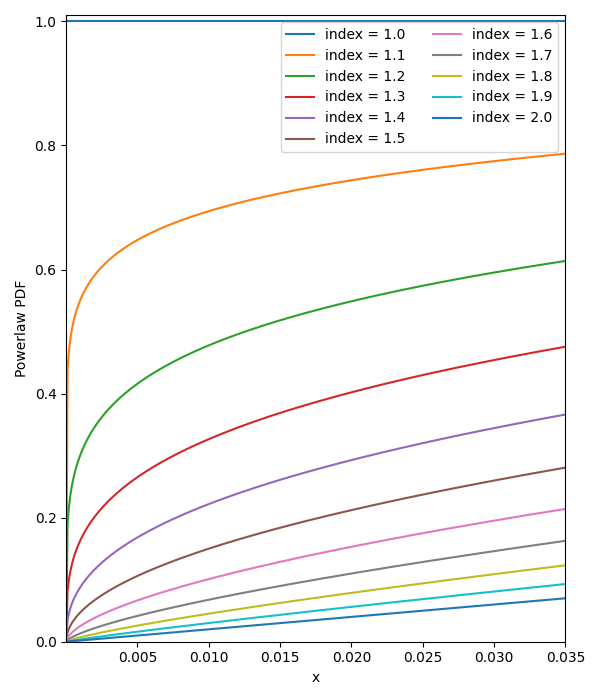
\includegraphics[width=\textwidth]{images/powerlaw}
    \captionof{figure}{Power law distribution}
\end{minipage}

\,\\\subsubsection*{\textbf{Beta distribution}}
For the beta distribution, we use the following form,
\begin{equation}
    f(x, a, b) = \frac{\Gamma(a+b)x^{a-1}(1-x)^{b-1}}{\Gamma(a)\Gamma(b)}
    \label{eq:beta_distribution}
\end{equation}
For $0 \leq x \leq 1, a > 0, b > 0$ and $\Gamma$ is the gamma function.\footnote{\url{https://docs.scipy.org/doc/scipy/reference/generated/scipy.stats.beta.html}}

Figure~\ref{fig:beta1} shows the beta distribution with a fixed $\beta=80$.
Similarly, figure~\ref{fig:beta2} shows the beta distribution with a fixed $\alpha=5$.
For our case, we selected $\text{Beta}(5, 80)$ as our distribution of choice for metallicity and generated $10^7$ values between the COMPAS limits $10^{-4} < z < 0.03$. %The same value for metallicity was used for both stars as different metallicity scenario is highly unlikely.

\begin{figure}[!ht]%
    \centering
    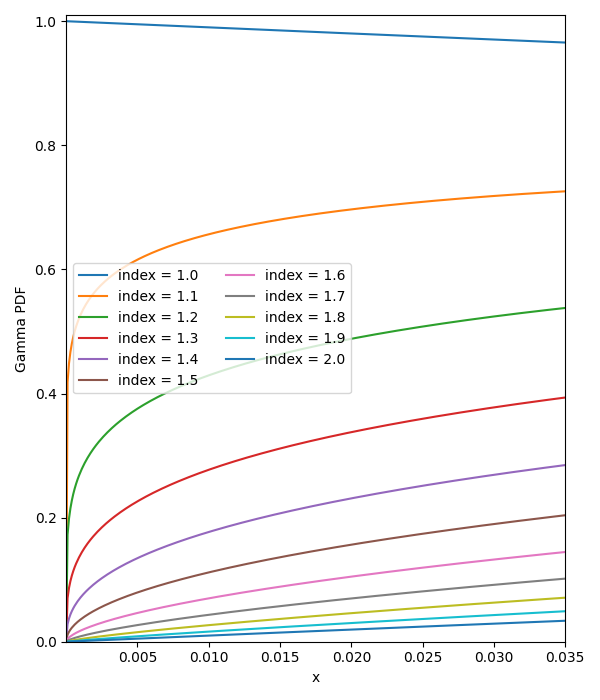
\includegraphics[width=\linewidth]{images/gamma}
    \caption{Gamma distribution with $1 \leq a \leq 2$.}
    \label{fig:gamma_distribution}
\end{figure}%
\begin{figure}[!ht]%
    \centering
    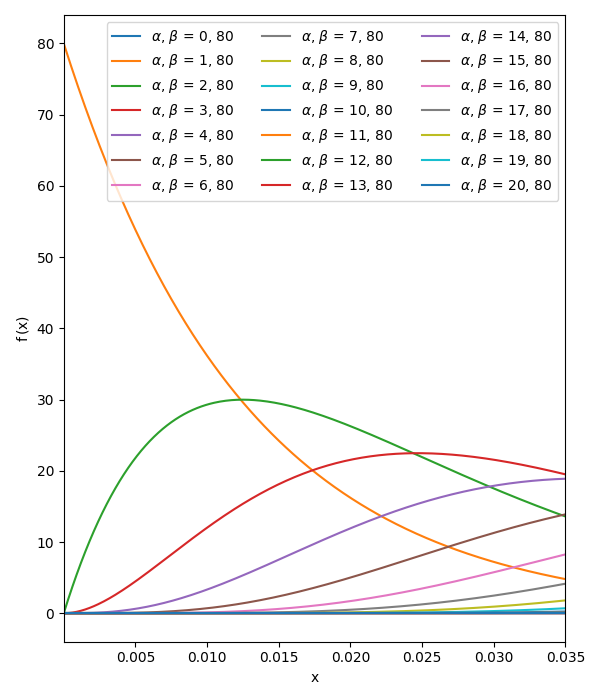
\includegraphics[width=\linewidth]{images/beta1}
    \caption{Beta distribution with varying $\alpha$ and fixed $\beta$ parameter.}
    \label{fig:beta1}
\end{figure}%
\begin{figure}[!ht]%
    \centering
    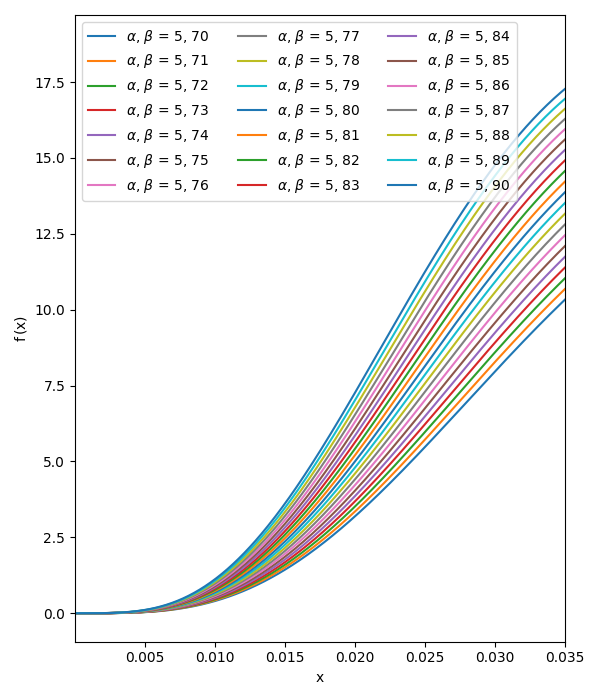
\includegraphics[width=\linewidth]{images/beta2}
    \caption{Beta distribution with fixed $\alpha$ and varying $\beta$ parameters.}
    \label{fig:beta2}
\end{figure}%

\subsection{\textbf{Metallicity}}
\label{subsec:metallicity}
One of the major challenges in generation of the stellar binaries for this study was the selection of a distribution which will result in stars at the higher end of COMPAS metallicity boundary, $z = 0.03$.
A power-law, gamma, and beta distributions were selected to try and simulate the required metallicity distribution.
In the following section, we discuss the selected distributions briefly,

\end{document}
